% begin module sequence-geometric-ex10
\begin{frame}
\begin{example} %[Example 10, p. 717]
\begin{columns}[c]
\column{.6\textwidth}
For what values of $r$ is the sequence $\{ r^n\}$ convergent?

\uncover<2->{%
Consider the exponential function $y = r^x$.}%
\abovedisplayskip=0pt
\belowdisplayskip=0pt
\[
\uncover<2->{%
\lim_{x\to\infty}r^x = \left\{ \begin{array}{lll}
\uncover<4->{\alert<handout:0| 4>{\infty}} & \alert<handout:0| 3-4>{\textrm{ if }} & \alert<handout:0| 3-4>{r > 1}\\
\uncover<6->{\alert<handout:0| 6>{0}} & \alert<handout:0| 5-6>{\textrm{ if }} & \alert<handout:0| 5-6>{0 < r < 1}\\
\end{array}\right.}%
\]
\uncover<7->{Therefore}
\abovedisplayskip=0pt
\belowdisplayskip=0pt
\[
\uncover<7->{%
\lim_{n\to\infty}r^n = \left\{ \begin{array}{lll}
\uncover<8->{\alert<handout:0| 8>{\infty}} & \alert<handout:0| 7-8>{\textrm{ if }} & \alert<handout:0| 7-8>{r > 1}\\
\uncover<10->{\alert<handout:0| 10>{0}} & \alert<handout:0| 9-10>{\textrm{ if }} & \alert<handout:0| 9-10>{0 < r < 1}\\
\end{array}\right.}%
\]
\uncover<11->{Also, $\displaystyle \alert<handout:0| 11-12>{\lim_{n\to\infty}1^n = \uncover<12->{1}}$ and $\displaystyle \alert<handout:0| 13-14>{\lim_{n\to\infty}0^n = \uncover<14->{0}}$.}

\uncover<15->{If $-1 < r < 0$, then $0 < |r| < 1$, and
\abovedisplayskip=0pt
\belowdisplayskip=0pt
\[
\lim_{n\to\infty} |r^n| = \lim_{n\to\infty}|r|^n = 0 
\]
Therefore $\displaystyle \lim_{n\to\infty}r^n = 0$.}

\uncover<16->{If $r < -1$, then $r^n$ diverges, just like $(-1)^n$.}
\column{.4\textwidth}
\ \only<handout:0| -7>{%
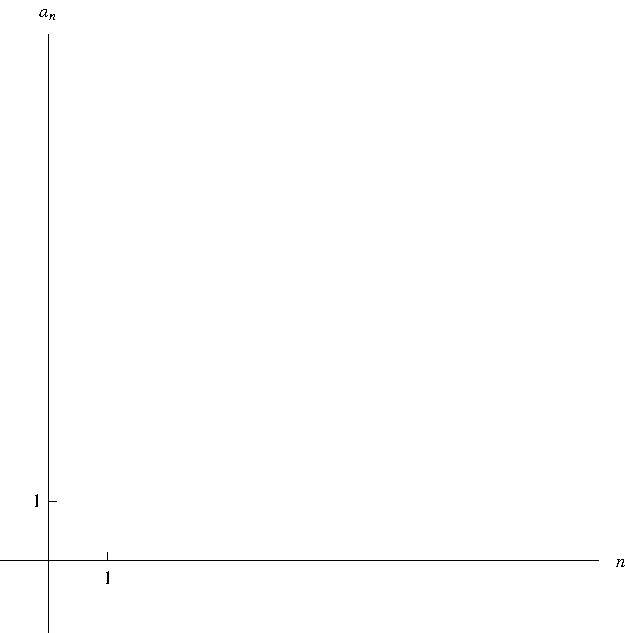
\includegraphics[height=3.8cm]{sequences/pictures/12-01-ex10a.pdf}%
}%
\only<handout:0| 8-9>{%
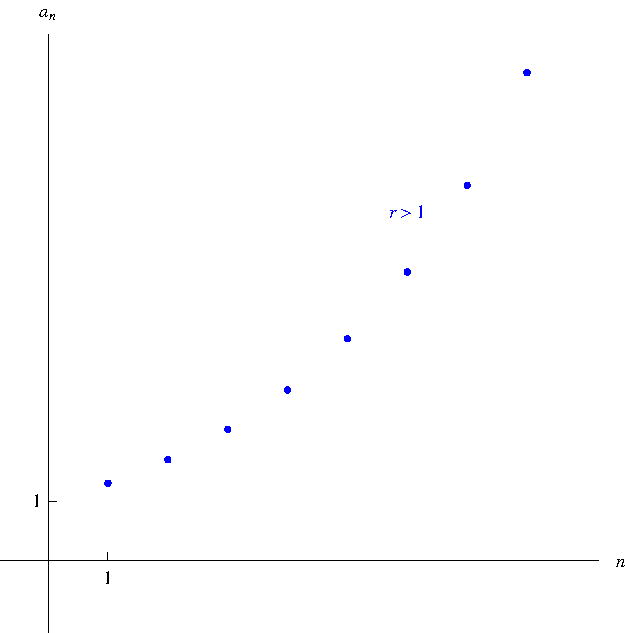
\includegraphics[height=3.8cm]{sequences/pictures/12-01-ex10b.pdf}%
}%
\only<handout:0| 10-11>{%
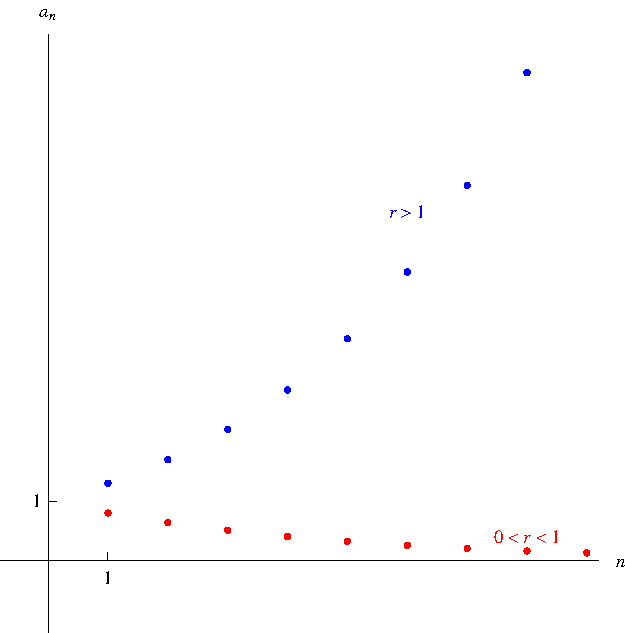
\includegraphics[height=3.8cm]{sequences/pictures/12-01-ex10c.pdf}%
}%
\only<12->{%
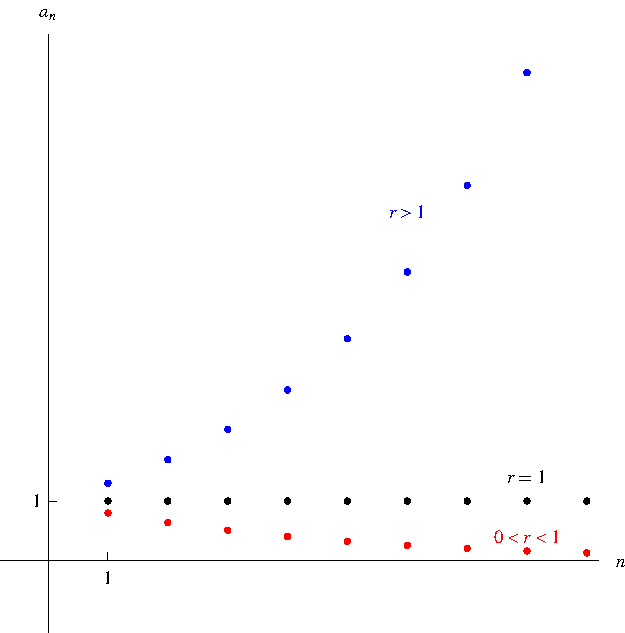
\includegraphics[height=3.8cm]{sequences/pictures/12-01-ex10d.pdf}%
}%

\ \only<handout:0| -14>{%
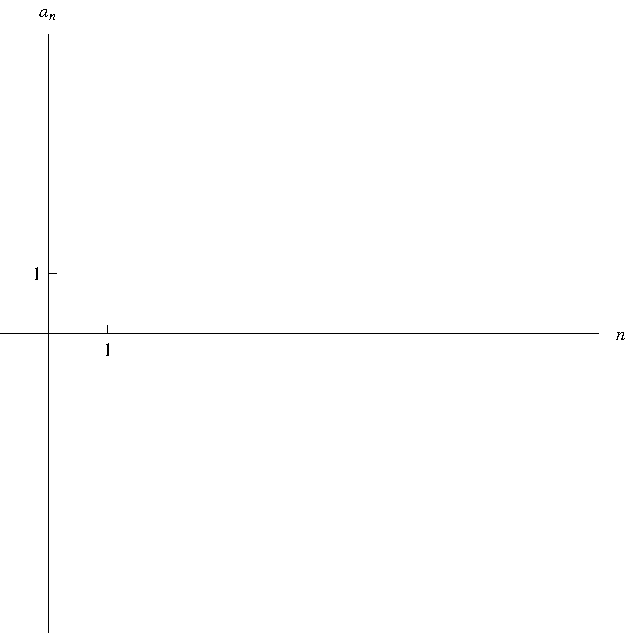
\includegraphics[height=3.8cm]{sequences/pictures/12-01-ex10e.pdf}%
}%
\only<handout:0| 15>{%
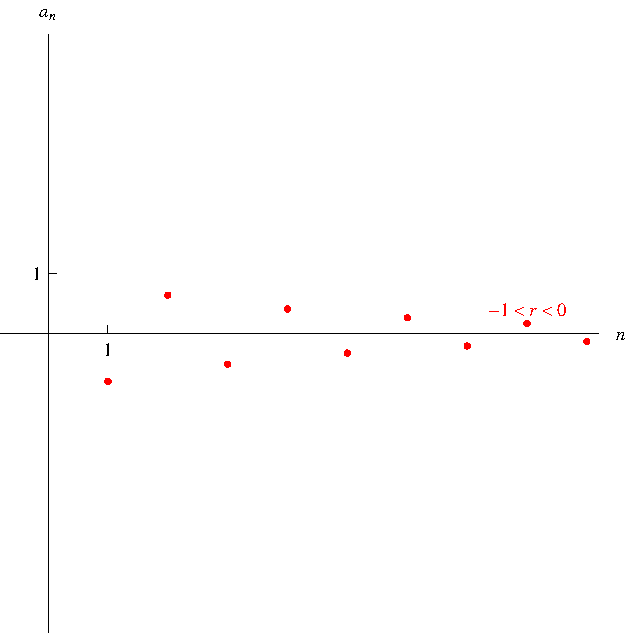
\includegraphics[height=3.8cm]{sequences/pictures/12-01-ex10f.pdf}%
}%
\only<16->{%
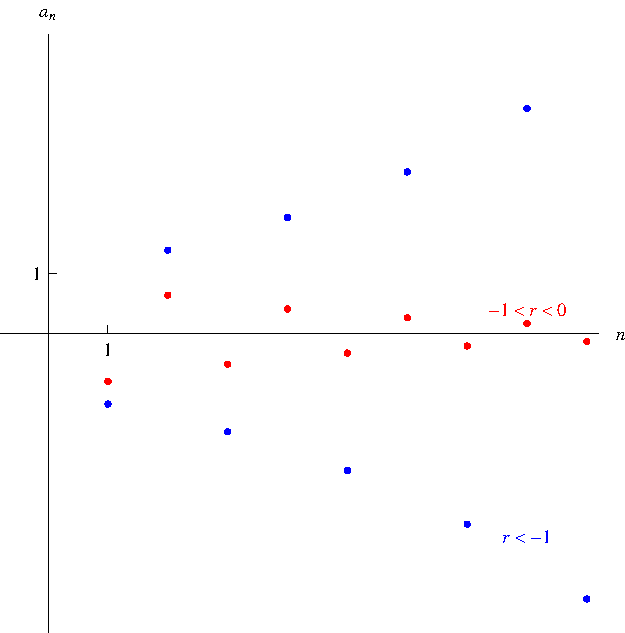
\includegraphics[height=3.8cm]{sequences/pictures/12-01-ex10g.pdf}%
}%
\end{columns}
\end{example}
\end{frame}
% end module sequence-geometric-ex10
